% !TEX root = ../thesis.tex
    
%**************************************************************
% MSCRED
%**************************************************************

\subsection{Multi-Scale Convolutional Recurrent Encoder-Decoder}
    MSCRED\cite{mscred} è un recente modello avanzato che si concentra sull'identificazione di anomalie all'interno di serie 
    temporali multivariate.

    \paragraph{Scelta del modello} MSCRED è stato scelto per diverse ragioni; come attestano gli autori del paper,
    è in grado di catturare informazioni a diverse scale temporali, grazie all'incorporazione di strati convoluzionali. 
    Inoltre, la sua architettura di codifica-decodifica è adatta per l'identificazione di pattern complessi. Fondamentalmente, 
    il modello è stato sviluppato con l'obiettivo specifico di gestire l'intercorrelazione dei segnali e la 
    dipendenza temporale tra di essi. Lo scopo principale è valutare se questo approccio avanzato possa migliorare 
    significativamente il rilevamento delle anomalie rispetto a modelli più tradizionali come 
    ARMA\cite{arma} e OC-SVM\cite{ocsvm}.
    
    
    \paragraph{Le controversie sul modello} L'implementazione originale, disponibile su 
    GitHub\footnote{\url{https://github.com/7fantasysz/MSCRED}}, non è stata accolta con entusiasmo dalla critica online. 
    Purtroppo, di per sé, il codice non è molto intuibile e sono presenti 
    dei riferimenti agli ambienti locali dello sviluppatore originale. Inoltre, nell'implementazione originale, le etichette
    che rappresentano le anomalie nel dataset non sono state fornite, rendendo impossibile replicare i risultati del paper.
    Tutto questo ha fatto suscitare dubbi riguardo all'effettiva efficacia del modello. Nella repository 
    GitHub\footnote{\url{https://github.com/Pikarz/tirocinio\_infostud}} relativa agli studi affrontati in questa relazione viene 
    allegata la versione del codice revisionata e rinnovata a fondo dal sottoscritto con cui sono stati effettuati gli esperimenti.


    \paragraph{Il framework del modello}
    Per quanto riguarda il modello in sé, le "signature matrices" sono una parte fondamentale di MSCRED e svolgono un 
    ruolo chiave nell'analisi delle serie temporali. Queste matrici sono utilizzate per rappresentare le intercorrelazioni
    tra diverse coppie di serie temporali in un segmento specifico della serie, una proprietà critica che riflette lo
    stato del sistema.
    

    Le signature matrices sono matrici $n \times n$ dove $n$ è il numero di segnali della serie temporale analizzata.
    Una certa signature matrix $M^t$ è costruita attraverso il prodotto interno di due serie temporali all'interno del segmento 
    interessato. Formalmente, date due serie temporali $\mathbf{x}^w_i = (x^{t-w}_i, x^{t-w-1}_i, \dots, x_i^t)$ e $\mathbf{x}_j^w =
    (x_j^{t-w}, x_j^{t-w-1}, \dots, x_j^t)$ appartenenti allo stesso segmento $X^w$, la loro correlazione $m_{ij}^t \in M^t$ è 
    calcolata secondo l'\hyperref[eq:sign-matr]{equazione 3.3.}

    \begin{equation}\label{eq:sign-matr}
        m_{ij}^t =\frac{\sum_{\delta=0}^w x_i^{t-\delta}x_j^{t-\delta}}{w}
    \end{equation}
            
    \begin{figure}[H]
        \centering
        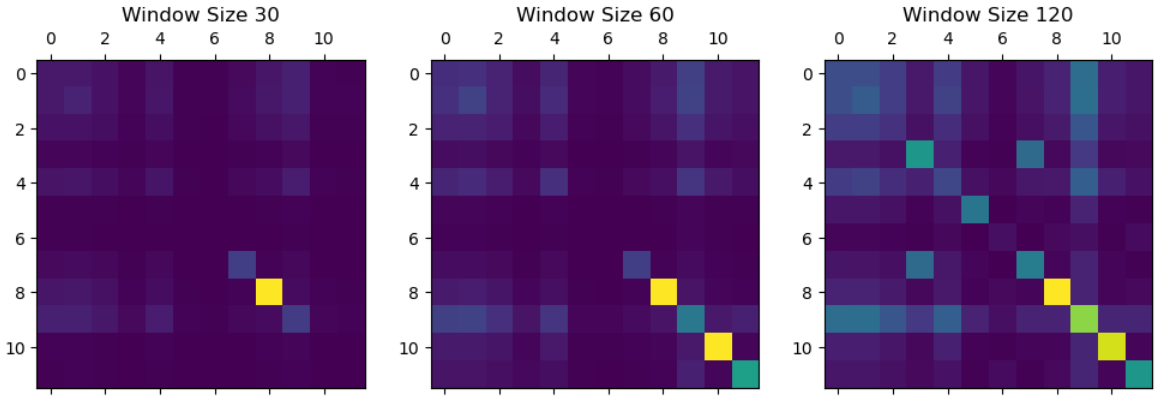
\includegraphics[width=0.6\textwidth]{./input/chapters/models/figs/signature_matrices.png}
        \caption{Signature matrices.} % Use caption to create a caption
        \label{fig:signature-matrices}
    \end{figure}

    Banalmente, le signature matrices sono matrici simmetriche. Nell'esperimento, l'intervallo tra due segmenti è 
    $gap\_time = 30$ e vengono costruite $s=3$ signature matrices con grandezze diverse pari a $win\_sizes = [30, 60, 120]$ punti
    temporali.
    Nella \hyperref[fig:signature-matrices]{Figura 3.8.} è illustrato un esempio di tre signature matrices su cui si
    basano i risultati dell'esperimento riportati nella \hyperref[val-mscred]{Sezione 4.5}.

    In sintesi, le signature matrices vengono concatenate e il tensore risultante $\chi^{t,0} \in \mathbb{R}^{n \times n \times s}$ 
    viene fornito in input a vari strati convoluzionali. Sia $\chi^{t,l}$ la feature map del livello $l$-esimo, attraverso un 
    attention based ConvLSTM\cite{convlstm} vengono aggiornati gli strati nascosti delle feature map $\mathcal{H}^{t,l}$ in $\hat{\mathcal{H}}^{t,l}$. 
    In seguito, attraverso un decodificatore convoluzionale, le feature map ottenute al passo precedente vengono decodificate e
    vengono ricostruite le signature matrices facendo, essenzialmente, il processo inverso: la feature map $\hat{\mathcal{H}}^{t,l}$ 
    viene data in input a una rete neurale deconvoluzionale e l'output, la feature map $\hat{\chi}^{t,l}$, è concatenato 
    con l'output del precedente layer convoluzionale. La concatenazione è poi data in input al prossimo strato deconvoluzionale. 
    L'output finale $\hat{\chi}^{t,0}$ denota le signature matrices ricostruite. La funzione di loss di MSCRED, osservabile
    nell'\hyperref[eq:mscred-loss]{equazione 3.4}, osserva la differenza tra le signature matrices originali e quelle ricostruite e, 
    nel corso delle epoche di training, punta a minimizzare tale funzione di loss.       

    \begin{equation}\label{eq:mscred-loss}
        \mathcal{L}_{MSCRED} = \sum_t \sum_{c=1}^s \Vert \chi^{t,0}_{:,:,c} - \hat{\chi}^{t,0}_{:,:,c} \Vert^2_F
    \end{equation}



    \paragraph{Il dataset} La suddivisione del dataset negli insiemi di training, validazione e test ha mantenuto 
    gli indici di suddivisione usati nell'esperimento di OC-SVM, osservabile nella 
    \hyperref[tab:dataset-ocsvm]{Tabella 3.2.}

    \paragraph{Iperparametri} MSCRED, come già anticipato nei paragrafi precedenti, presenta diversi iperparametri, tra cui 
    $win\_sizes$ che rappresenta la larghezza delle signature matrices, $gap\_time$, che determina la distanza tra i segmenti 
    della serie temporale, ovvero identifica quanto scorre ogni finestra a ogni passo, e $s$ che è il numero signature matrices. 
    Inoltre, l'iperparametro $step\_max$ rappresenta il numero di feature maps precedenti 
    concatenate dal codificatore convoluzionale e $thred\_b$ e $threshold$ regolano la sensibilità del modello 
    nel determinare le anomalie. In particolare, $thred\_b$ rappresenta un valore di soglia specifico utilizzato 
    dal modello per valutare numericamente l'indice di anomalia degli elementi all'interno dei dati, associando a essi
    un certo punteggio di anomalia. $threshold$, invece, è atto a valutare le prestazioni complessive 
    del modello e stabilisce una soglia oltre la quale i punteggi di anomalia vengono etichettati come anomalie.

    Dopo un'attenta analisi sono stati scelti per l'esperimento gli iperparametri riportati nella 
    \hyperref[tab:mscred-iperparams]{Tabella 3.6.} che hanno garantito la migliore soluzione
    empirica. I restanti iperparametri $thred\_b$ e $threshold$, sono stati ottimizzati tramite una grid-search atta 
    a massimizzare la metrica F1.

    \begin{table}[H]
        \centering
        \caption{Iperparametri MSCRED (parte 1.)}
        \begin{tabular}{lc}
            \toprule
            \textbf{Iperparametro} & \textbf{Valore} \\
            \toprule
            $win\_sizes$ & $30, 60, 120$ \\
            $s$ & $3$ \\
            $step\_max$ & $20$ \\
            $gap\_time$ & $30$ \\
            \bottomrule
        \end{tabular}
        \label{tab:mscred-iperparams}
    \end{table}

    Formalmente, siano $\mathbf{Tr}, \mathbf{Va}$ i dataset utilizzati per il training e
    per il validation rispettivamente, e sia $\text{MSCRED}_\mathbf{X}^\mathbf{Y}$ un modello MSCRED addestrato con gli iperparametri 
    della \hyperref[tab:mscred-iperparams]{Tabella 3.6.} su $\mathbf{X}$ che effettua previsioni nei punti $\mathbf{Y}$, 
    e sia $thred\_bs_{50}$ uno spazio lineare costituito da elementi equidistanti $thred\_b_i$ tali che $thred\_b_i \in 
    [1\mathrm{e}{-11}, 1\mathrm{e}{-6}] \forall i \in [50]$ e sia 
    $Thres$ la lista esaustiva dei possibili threshold, ovvero dei vari anomaly score $V_{\text{score}}$, 
    generati dal modello per ogni punto:

    \begin{equation}
        \label{eq:mscred-problem}
        \begin{aligned}
            & thred\_b^*, threshold^* = \max_{\substack{thred\_b, \\ threshold}} F1(\text{MSCRED}_\mathbf{Tr}^\mathbf{Va}(thred\_b, threshold)) \\
            & \text{con il vincolo} \quad thred\_b \in thred\_bs_{50}, threshold \in V_{\text{score}}
        \end{aligned}
    \end{equation}

    \begin{table}[H]
        \centering
        \caption{Iperparametri MSCRED (parte 2.)}
        \begin{tabular}{lc}
            \toprule
            \textbf{Iperparametro} & \textbf{Valore} \\
            \toprule
            $thred\_b^*$ & $6.326$ \\
            $threshold^*$ & $134.747$ \\
            \bottomrule
        \end{tabular}
        \label{tab:mscred-iperparams2}
    \end{table}
    Gli iperparametri che hanno soddisfatto l'\hyperref[eq:mscred-problem]{equazione 3.5} sono riportati nella 
    \hyperref[tab:mscred-iperparams2]{Tabella 3.7.}

    È bene notare che un numero di passaggi temporali pari a $gap\_time$ vengono collassati in uno singolo dopo la computazione di MSCRED,
    quindi data una serie temporale che contiene $x$ osservazioni, la soluzione generata avrà $x \bmod gap\_time$ osservazioni.